

\vspace{-\baselineskip}
\paragraph{Projection across entailment-cancelling operators.}  \hspace{-1em}
	Attitude ascriptions may come with an inference to the truth of their complement, which can project across entailment-cancelling operators (illustrated for \emph{\lq discover\rq} in \ref{ex:family}) \citep[et seq.]{kiparsky_fact_1970}.


	\vspace{-.4\baselineskip}
	% The semantically heterogeneous entailment-cancelling operators are still often assumed to have similar effects on projection (xxx references xxx).
	\citet{karttunen_observations_1971} proposed that projective triggers differ in how their projection behavior is affected by the different embedding contexts in \ref{ex:family}, distinguishing \emph{factive} predicates (\emph{regret, forget, resent}) from \emph{semi-factive} predicates (\emph{discover, realize, see, find out, notice}), suggesting that the content of factive complements always projects, while for semi-factives it does not always do so in polar questions or conditional antecedents \citep[see also][]{stalnaker_pragmatic_1977}. Throughout the literature, this distinction is often understood in terms of emotive factive and cognitive semi-factive predicates \citep{klein_two_1975,djarv_cognitive_2018}, suggesting that emotive factives indifferently project across entailment-cancelling operators, while cognitive semi-factives project only when asserted or denied.
	Although widely assumed, there has been little experimental evidence or systematic investigation to support Karttunen's intuition.

	% Previous work on projection showed that it is not a categorial property of lexical triggers \citep{tonhauser_how_2018}, but a gradient one, affected by various contextual factors \citep{simons_what_2010,de_marneffe_did_2012,beaver_questions_2017,degen_prior_2021}. In light of this, we expect that the hetergeneous entailment-cancelling operators in \ref{ex:family} affect projection differentially.
	%

	%
	% To provide a systematic way of distinguishing these classes, \cite{djarv_cognitive_2018} suggest that they correspond to emotive and cognitive predicates, respectively. In a study assessing the acceptability of affirmative responses to a target utterance while explicitly denying a potentially projective inference \citep[based on][]{cummins_experimental_2012}, they find that this kind of affirmative cancellation is more readily available for emotive than cognitive predicates, suggesting that the main clause content and projective content are logically more independent from each other for emotive predicates.
	%

	\cite{smith_relationship_2014}, investigating the effect of operator for various types of projection triggers on ratings of surprisal about the inferences in question, conclude that inferences triggered by \emph{know} and epithets project more from under negation than conditional antecedents whereas non-restrictive relative clauses show the opposite pattern.

	Here, we analyze measures from a task designed to assess speaker commitment more directly to address the questions: \textbf{(i)} Is projection affected by differences in entailment-canceling environments? \textbf{(ii)} Do these effects vary for different attitude verb triggers (and in what way)? A complex picture of projection emerges, with interactions beween entailment-canceling operators and triggers, not yet suggested in the literature. Our results indicate a need for a more nuanced view of the family-of-sentences diagnostics of projection, as well as a better understanding of the effect of the interaction between lexical semantics and operators on projection.

\vspace{-\baselineskip}
\paragraph{Experiments.} \hspace{-1em}
	We use the data from 12 experiments, which consisted of two blocks each: a projection task and a at-issueness task. These experiments were initially designed to investigate three at-issueness diagnostics (with sentences under each of the four entailment-canceling operations, for a total of 12 experiments) and their correlation to projection ratings. Here, we focus only on the projection data. To assess projection, we used a task eliciting responses about how strongly a speaker would be committed towards the embedded clause \citep[from][]{tonhauser_prosodic_2016}. We presented sentences like in \ref{ex:family} as uttered by a named speaker (e.g. “\textbf{Daniel:} \emph{\lq Did Cole\dots?\rq}”). Participants then provided a certainty-rating in response to a prompt like: \emph{“Is Daniel certain that Julian dances Salsa?”}, by moving a slider on a scale from \lq no\rq\ (coded as \texttt{0}), to \lq yes\rq\ (coded as \texttt{1}). 

% paragraph experiment (end)

\vspace{-\baselineskip}
\paragraph{Comparisons and Expectations.} \hspace{-1em}
	We compared certainty-ratings for the four entailment-canceling operators in \ref{ex:family} (factor \texttt{operator}), and 20 clause-embedding predicates (factor \texttt{verb}: {\em be annoyed, discover, know, reveal, see, acknowledge, admit, announce, confess, confirm, establish, hear, inform, prove, pretend, suggest, say, think, be right, demonstrate}).
	Based on the Karttunen-Klein hypothesis about emotive factives vs. cognitive semi-factives, we would expect emotive factives (\emph{be annoyed}), and verbs normally taken to be factive (\emph{know}), to be highly projective in a way that is indifferent to the embedding context, and cognitive semi-factives (\emph{discover, see}) to show higher projectivity ratings under negation compared to questions and conditionals.

% paragraph design_and_expectations_ (end)

\vspace{-\baselineskip}
\paragraph{Method.} \hspace{-1em}
	The 12 experiments in our study all manipulated the factor \texttt{verb} for 20 items corresponding to to the content of the complement clause. Experiments 1--3 used polar question embedding, exps. 4--6 used negation, 7--9 modals, and 10--12 conditionals, making the \texttt{operator} manipulation a between-subjects factor. We analyzed data from $2682$ self-identified native English speakers participated online across the 12 experiments (recruited via Prolific and Amazon MTurk). Participants saw items Latin-squared and randomized with six control stimuli.

% paragraph method (end)

\vspace{-\baselineskip}
\paragraph{Results and Discussion.} \hspace{-1em}
	Pooling the data across our experiments, we examined the effect on certainty-ratings of \texttt{operator}, and \texttt{verb}, as well as their interaction. Mean certainty-ratings by operator and predicate, and 95\% bootstrapped confidence intervals are given in  \textbf{Figure \ref{fig:figure1}}. 

	% \vspace{-.3\baselineskip}
	% \textbf{version w baseline know/m}
	% \noindent The data was analyzed using a mixed effects linear regression (using \texttt{lme4, lmertest} in \texttt{R}; \citealp{bates_fitting_2015,kuznetsova_lmertest_2016,r_core_team_r_2014}), with \texttt{know} and \texttt{modal} as reference levels, and random intercepts for participants and items. We found highly significant main effects of \texttt{operator} (\texttt{conditional}: $+0.142$, \texttt{negation}: $+0.143$, ; \texttt{question}: $+0.225$, where $p < 2e^{-16}$ in all three cases), as well as many interactions of \texttt{operator} and  \texttt{verb} across the board (where $p < 0.001$ in $38$ cases, $p < 0.01$ in one, and $p < 0.05$ in three out of $57$ possible interactions).\\

	The data was analyzed using a mixed effects linear regression (using \texttt{lme4, lmertest} in \texttt{R}; \citealp{bates_fitting_2015,kuznetsova_lmertest_2016,r_core_team_r_2014}), with \texttt{be\_annoyed} and \texttt{negation} as reference levels, and random intercepts for participants and items.
	% The mean for this baseline (intercept) is $0.867$.
	We found highly significant main effects of \texttt{operator}: For our baseline \texttt{be\_annoyed}, both \texttt{conditional} and \texttt{modal} are clearly less projective than negation, thereby supporting the claim that the embedding context does matter. We also found many interactions of \texttt{operator} and \texttt{verb} across the board, suggesting that the effect of embedding context diffes by verb. 

	Notably, for the emotive predicate \emph{\lq be annoyed\rq}, we found no significant difference between question and negation contexts, as would be expected based on Karttunen, but unexpectedly, we find lower ratings for conditionals and modals compared to negation. The cognitive predicate \emph{\lq discover\rq}, is more projective in polar questions and conditional antecedents than under negation, patterning opposite to Karttunen's claims about semi-factives. The predicate \emph{know}, which is often regarded a canonical factive, shows effects that would be incompatible with a characterization as either factive or semi-factive: $\texttt{question} > \texttt{conditional, negation} > \texttt{modal}$. If \emph{\lq know\rq} is a factive predicate, no difference would be expected here. If it is semi-factive, we would, again, expect higher projectivity under negation than in questions and conditionals.

	% for \texttt{conditional} ($-0.116$, $p < 1.6e^{-13}$) and \texttt{modal} ($-0.156$, $p < 2e^{-16}$), while the effect of \texttt{question} was only marginally significant ($+0.025$, $p < 0.1$). We also found many interactions of \texttt{operator} and \texttt{verb} across the board (where $p < 0.001$ in $43$ cases, $p < 0.01$ in three, and $p < 0.05$ in one out of $57$ possible interactions).\\
	
% paragraph results (end)

\vspace{-\baselineskip}
\paragraph{Verb profiles.} % (fold)
	\textbf{Figure \ref{fig:figure2}} gives the mean certainty ratings for the four operators by predicate, showing different predicate profiles. xxx analyses of the profiles xxx
% paragraph profiles (end)

\vspace{-\baselineskip}
\paragraph{Conclusion.} % (fold)
	\begin{itemize}
		\item Entailment-cancelling operators affect projection in different ways: calling into question the uniform applicability of the family-of-sentences diagnostic
		\item The effect of entailment-cancelling operator on projection differs for different verbs. The picture that emerges could not be characterized in terms of Karttunen's characterization of (semi)factives.
		\item We find some preliminary verb classes.
	\end{itemize}
% paragraph conclusion (end)

\pagebreak
\begin{figure}[t]
		\vspace{-.8\baselineskip}
		\centering
		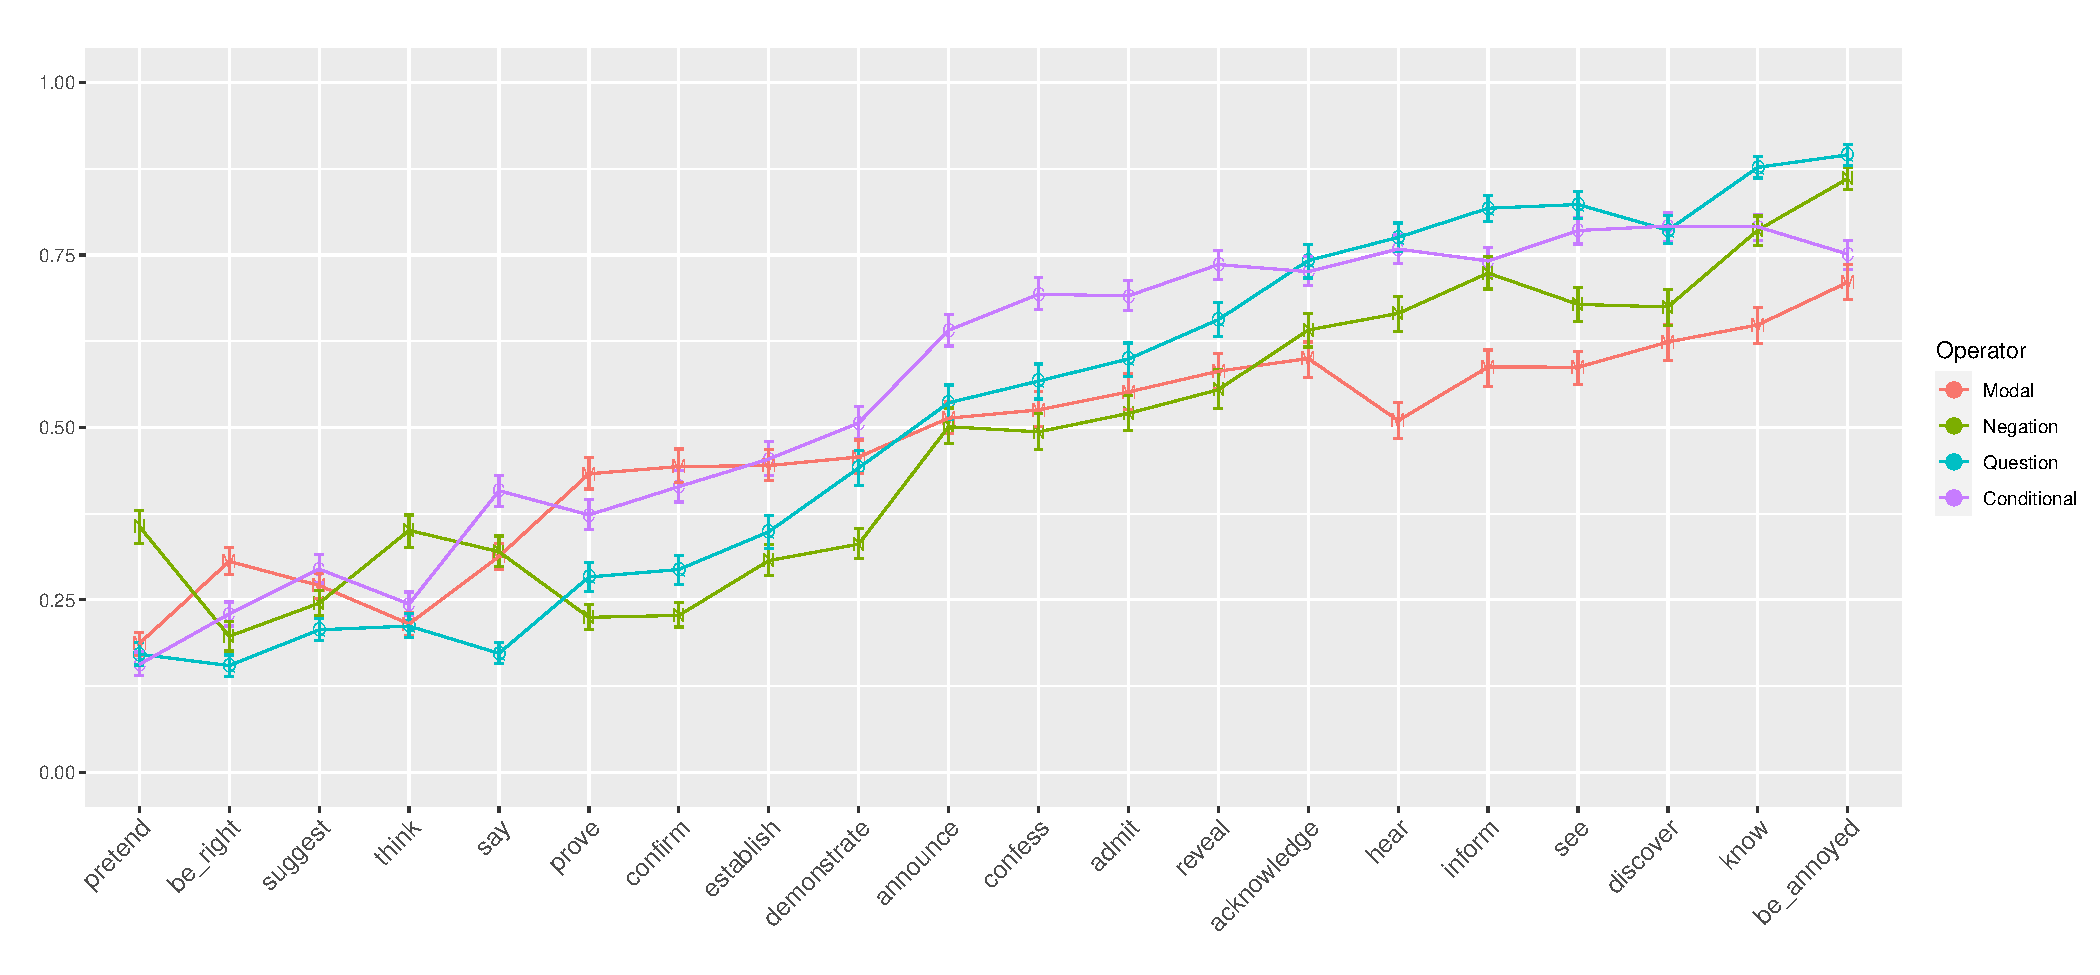
\includegraphics[width=\textwidth]{graphs/proj-by-both.pdf}\vspace{-1.2\baselineskip}
		\caption{\small Mean certainty ratings by predicate and operator with 95\% bootstrapped confidence intervals (y-axis), by verb (x-axis), and operator (color/grouping, where: \texttt{N} (blue): negation, \texttt{M} (green): modals, \texttt{C} (red): conditional antecedents, \texttt{Q} (purple): polar questions).}
		\label{fig:figure1}
	\end{figure}

	\begin{figure}[ht]
		\vspace{-.8\baselineskip}
		\centering
		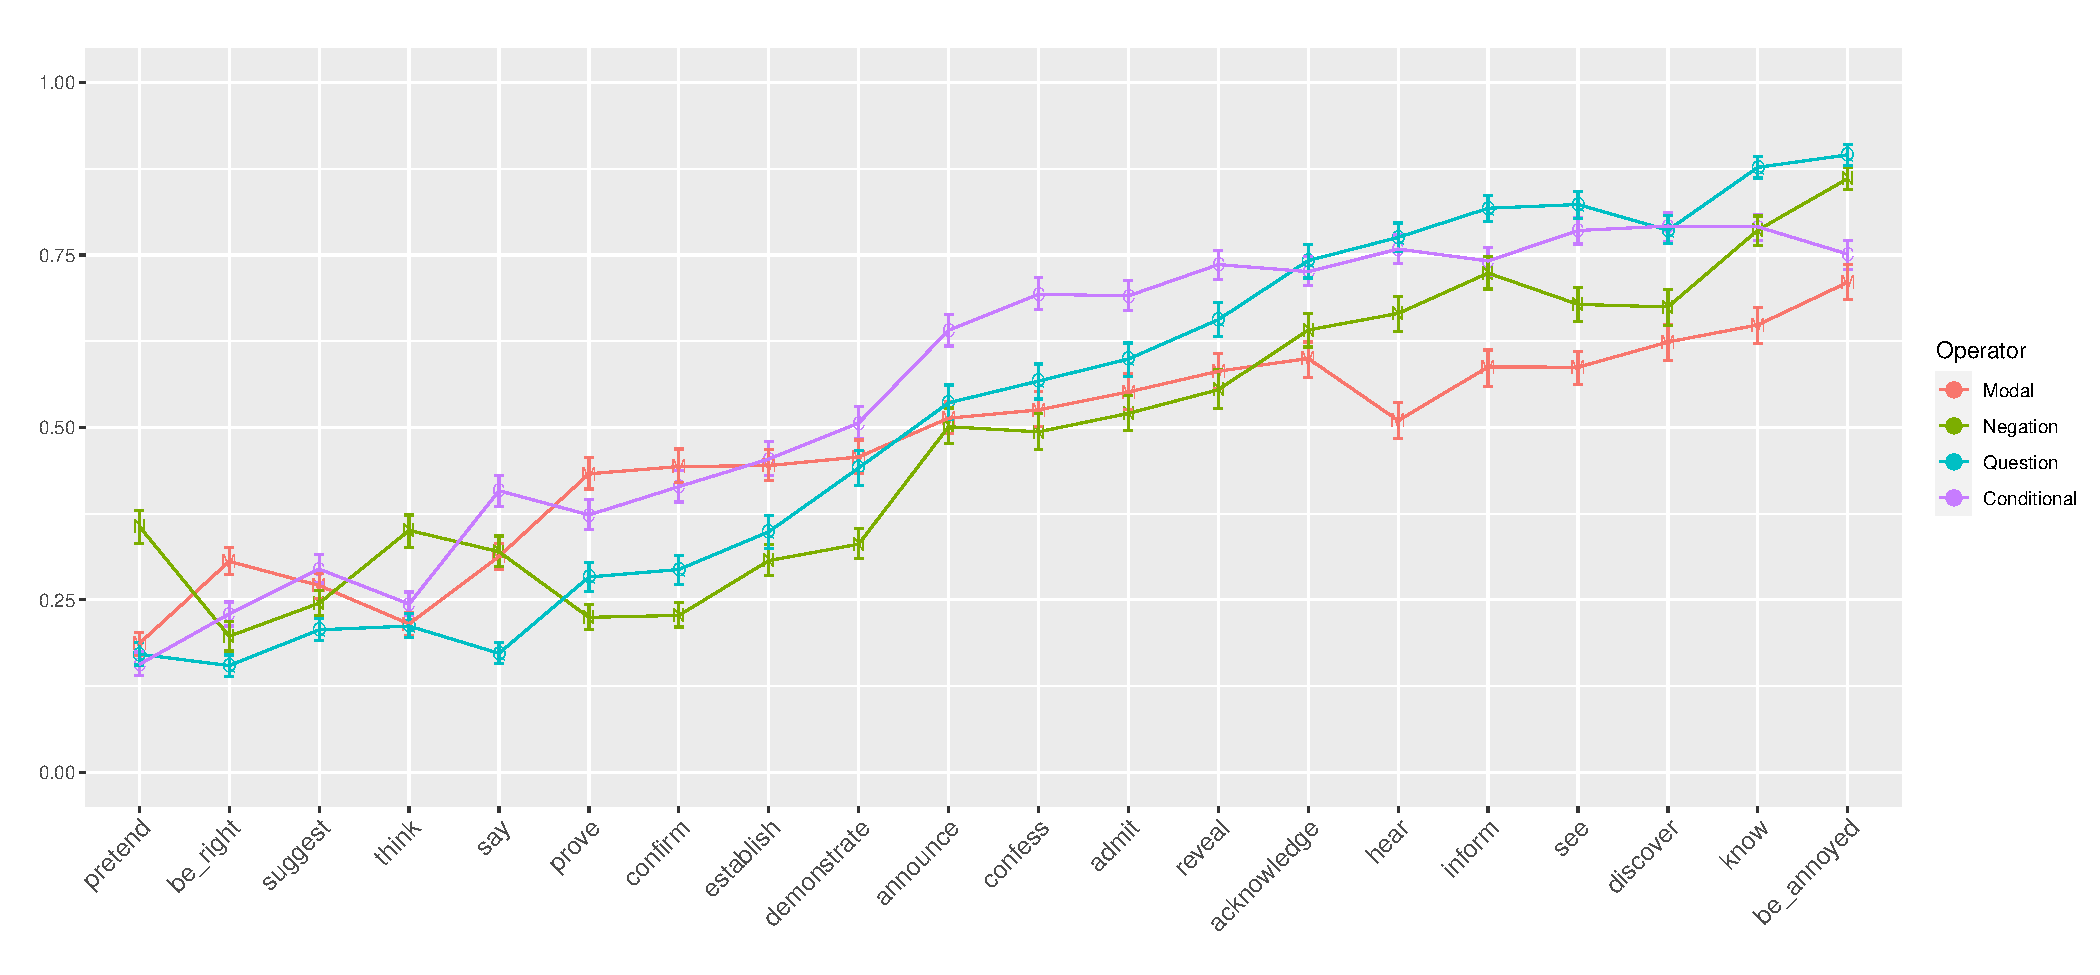
\includegraphics[width=\textwidth]{graphs/proj-by-both.pdf}\vspace{-1.2\baselineskip}
		\caption{\small Mean certainty ratings by predicate and operator with 95\% bootstrapped confidence intervals (y-axis), by verb (x-axis), and operator (color/grouping, where: \texttt{N} (blue): negation, \texttt{M} (green): modals, \texttt{C} (red): conditional antecedents, \texttt{Q} (purple): polar questions).}
		\label{fig:figure2}
	\end{figure}

\bibliography{projective-content.bib}

\end{document}